% --------------------------------------------------------------------------------

\begin{exercise}

\phantom{}

\begin{enumerate}[label = (\roman*)]

    \item Lösen Sie das Randwertproblem für die Laplacegleichung in ebenen Polarkoordinaten
    
    \begin{align*}
        (\Delta u)(r, \varphi)
        & =
        0 ~\text{für}~ r < R, \\
        u(R, \varphi)
        & =
        f(\varphi) ~\text{für alle}~ \varphi,
    \end{align*}

    wobei

    \begin{align*}
        \Delta u
        =
        u_{rr} + \frac{1}{r} u + \frac{1}{r^2} u_{\varphi \varphi}
    \end{align*}

    der Laplaceoperator in Polarkoordinaten, $R > 0$ eine positive Konstante und $f$ eine stückweise stetig differenzierbare $2 \pi$-periodische Funktion ist?

    \item Wie sieht die Lösung konkret im Fall
    
    \begin{align*}
        f(\varphi)
        =
        \begin{cases}
            0,  \varphi = 0, \pi \\
            1,  0 < \varphi < \pi \\
            -1, \pi < \varphi < 2 \pi
        \end{cases}
    \end{align*}

    mit $R = 1$ aus?

\end{enumerate}

\textit{Hinweis:}
Verwenden Sie einen Separationsansatz.
Betrachten Sie dazu zunächst Einzellösungen $u_n$ der Gestalt $u_n(r, \varphi) = v_n(r) \cdot w_n(\varphi)$ (mit $w_n$ $2 \pi$-periodisch), welche die Differentialgleichung erfüllen und insbesondere $C^2$ im Nullpunkt sind.
Die gesuchte Gesamtlösung ergibt sich dann als Summe über die Einzellösungen $u_n$ mit geeigneten Koeffizienten.
Falls Sie dabei auf die homogene eulersche Differentialgleichung 2. Ordnung stoßen, verwenden Sie Aufgabe 6 von Blatt 1 oder schlagen sie in einer beliebigen Quelle ein Fundamentalsystem von Lösungen nach.

\end{exercise}

% --------------------------------------------------------------------------------

\begin{solution}

\phantom{}

\begin{enumerate}[label = (\roman*)]

    \item Weil $f$ stückweise stetig differenzierbar und $2 \pi$-periodisch ist, hat es die Darstellung

    \begin{align*}
        f = \sum_{n=1}^N \1_{A_n} f_n,
        \quad
        N \in \N,
        \quad
        \bigcup_{n=1}^N A_n = [0, 2 \pi),
        \quad
        \Forall n = 1, \ldots, N:
        f_n |_{A_n} \in C^1.
    \end{align*}

    Wir folgen dem Hinweis, und betrachten die PDE einmal nur auf einem $A_n$ mit $n = 1, \ldots, N$.
    Sei $\varphi \in (0, 2 \pi]$ fest gewählt.
    Die Randbedingung und Separation geben uns

    \begin{align*}
        f_n(\varphi) = u_n(R, \varphi) = v_n(R) w_n(\varphi)
        \stackrel{!}{\implies}
        f_n^\primeprime(\varphi) = v_n(R) w_n^\primeprime(\varphi).
    \end{align*}

    Die Bedingung an den Laplaceoperator führt andererseits zu

    \begin{align*}
        0 \stackrel{!}{=}
        \Delta u_n
        =
        \pderivative[2]{r} (v_n w_n)
        +
        \frac{1}{r} \pderivative{r} (v_n w_n)
        +
        \frac{1}{r^2} \pderivative[2]{\varphi} (v_n w_n)
        =
        v_n^\primeprime w_n
        +
        \frac{1}{r} v_n^\prime w_n
        +
        \frac{1}{r^2} v_n w_n^\primeprime \\
    \end{align*}

    Jetzt multiplizieren wir mit $r^2 v_n(R)$ und \Quote{stoßen} auf eine \Quote{eulersche Differentialgleichung 2. Ordnung}.

    \begin{align*}
        \implies
        0 =
        r^2 v_n^\primeprime v_n(R) w_n
        +
        r v_n^\prime v_n(R) w_n
        +
        v_n v_n(R) w_n^\primeprime
        =
        f_n(\varphi) r^2 v_n^\primeprime
        +
        f_n(\varphi) r v_n^\prime
        +
        f_n^\primeprime(\varphi) r v_n
    \end{align*}

    Unsere \Quote{beliebige Quelle} an der Stelle ist (NATÜRLICH, was sonst?) Wikipedia!

    \begin{figure}[h!]
        \centering
        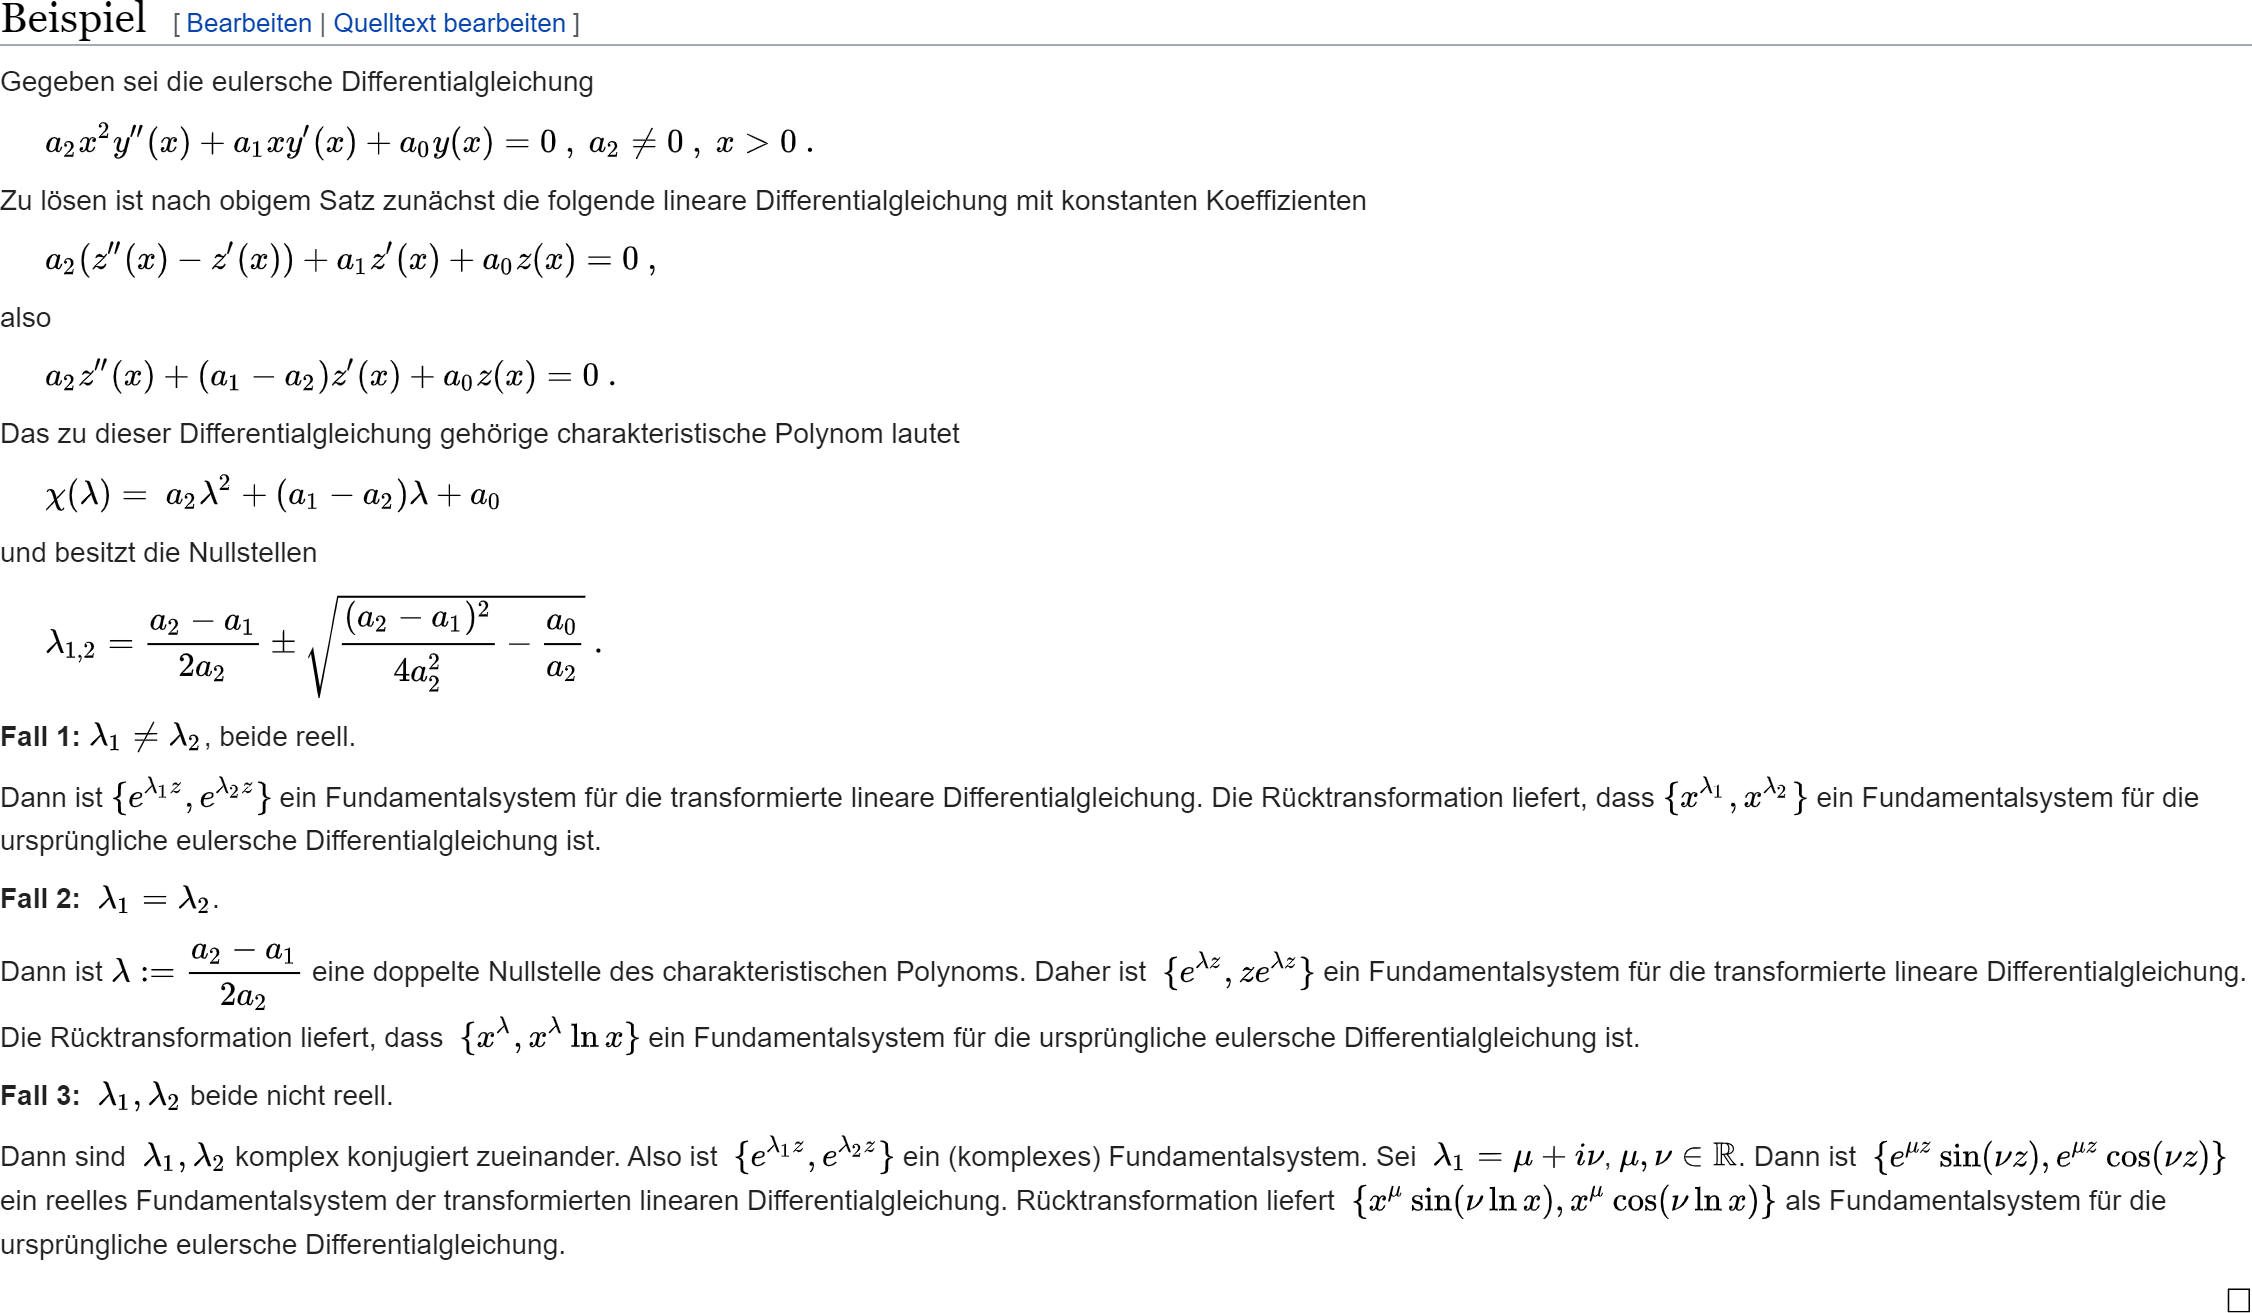
\includegraphics[width = \textwidth]{Euler Wikipedia.png}
        \caption{Click \href{https://de.wikipedia.org/wiki/Eulersche_Differentialgleichung}{here}!}
    \end{figure}

    ACHTUNG: Die Nullstellen hängen formal immer noch von $\varphi$ ab!

    \begin{align*}
        \lambda_n(\varphi)
        =
        \frac{f_n(\varphi) - f_n(\varphi)}{2 f_n(\varphi)}
        \pm
        \sqrt
        {
            \frac{(f_n(\varphi) - f_n(\varphi))^2}{4 f_n(\varphi)^2}
            -
            \frac{f_n^\primeprime(\varphi)}{f_n(\varphi)}
        }
        =
        \sqrt{-\frac{f_n^\primeprime(\varphi)}{f_n(\varphi)}}
    \end{align*}

    Wir machen die Fallunterscheidungen und bekommen ein Fundamentalsystem $V_{n, \varphi, 1}, V_{n, \varphi, 2}$.
    Wir wählen zwei beliebige Koeffizienten $c_{n, 1}, c_{n, 2} \in \R$ an.
    (Die hängen NICHT von $\varphi$ ab.)

    \begin{align*}
        v_{n, \varphi, c_{n, 1}, c_{n, 2}} = c_{n, 1} V_{n, \varphi, 1} + c_{n, 2} V_{n, \varphi, 2}
        & \implies
        w_{n, c_{n, 1}, c_{n, 2}}(\varphi) = \frac{f_n(\varphi)}{v_{n, \varphi, c_{n, 1}, c_{n, 2}}(R)} \\
        & \implies
        u_{n, \varphi, c_{n, 1}, c_{n, 2}}
        =
        v_{n, \varphi, c_{n, 1}, c_{n, 2}}
        w_{n, c_{n, 1}, c_{n, 2}}(\varphi)
        =
        \frac
        {
            f_n(\varphi)
            v_{n, \varphi, c_{n, 1}, c_{n, 2}}
        }{
            v_{n, \varphi, c_{n, 1}, c_{n, 2}}(R)
        }
    \end{align*}

    Diese Einzellösungen setzen wir nun zusammen.

    \begin{align*}
        u_c(r, \varphi)
        =
        \sum_{n=1}^N \1_{A_n} u_{n, \varphi, c_{n, 1}, c_{n, 2}},
        \quad
        c = ((c_{n, 1}, c_{n, 2}))_{n=1}^N
    \end{align*}

    \item 

    \begin{align*}
        f = \1_{(0, \varphi)} - \1_{(\pi, 2 \pi)}
        \implies
        \lambda_n = 0
        \implies
        V_{n, 1} = 1, V_{n, 2} = \ln{r}
        \implies
        v_n = c_{n, 1} + c_{n, 2} \ln
    \end{align*}

    \begin{align*}
        v_n(R)
        =
        c_{n, 1} + \underbrace{c_{n, 2} \ln{R}}_0
        \implies
    \end{align*}

    \begin{enumerate}

        \item \Quote{$\varphi = 0, \pi$}:
        \begin{align*}
            w_1(\varphi)
            =
            \frac{f_1(\varphi)}{v_1(R)} = 0
            \implies
            u_1 = 0
        \end{align*}

        \item \Quote{$0 < \varphi < \pi$}:
        \begin{align*}
            w_2(\varphi)
            =
            \frac{f_2(\varphi)}{v_2(R)}
            =
            \frac{1}{c_{1, 2}}
            \implies
            u_2(r, \varphi)
            =
            \frac{v_2(r)}{c_{1, 2}}
            =
            \frac{c_{1, 2} + c_{2, 2} \ln{r}}{c_{1, 2}}
            =
            1 + \underbrace{\frac{c_{2, 2}}{c_{1, 2}}}_{=: \eta} \ln{r}
        \end{align*}

        \item \Quote{$\pi < \varphi < 2 \pi$}:
        \begin{align*}
            w_3(\varphi)
            =
            \frac{f_3(\varphi)}{v_3(R)}
            =
            \frac{-1}{c_{1, 3}}
            \implies
            u_3(r, \varphi)
            =
            -\frac{v_3(r)}{c_{1, 3}}
            =
            -\frac{c_{1, 3} + c_{2, 3} \ln{r}}{c_{1, 3}}
            =
            -1 \underbrace{-\frac{c_{2, 3}}{c_{1, 3}}}_{=: \zeta} \ln{r}
        \end{align*}

    \end{enumerate}

    \begin{align*}
        \implies
        u(r, \varphi)
        =
        \begin{cases}
            0,                & \varphi = 0, \pi, \\
            \eta  \ln{r} + 1, & 0 < \varphi < \pi, \\
            \zeta \ln{r} - 1, & \pi < \varphi < 2 \pi
        \end{cases}
    \end{align*}

\end{enumerate}

\end{solution}

% --------------------------------------------------------------------------------
